\documentclass[../report.tex]{subfiles}
\begin{document}
\graphicspath{{img/}{../img/}}


Since all but one service operations on \textit{ShareIt} are private to clients, and some of these to users, it is important to discuss how access control is handled.

Two consecutive walls will block ones way when reaching \textit{ShareIt}; first a client token validation and secondly a user credential validation. \\

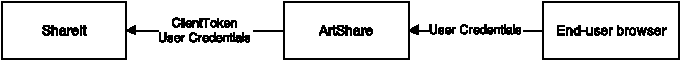
\includegraphics[width=\linewidth]{./AccessControlDeployment.pdf}

\subsection{Token validation}
\label{sec:Token}

The token validation is implemented as a means for \textit{ShareIt} to only allow recognized clients to invoke operations. This works because \textit{ShareIt} and a Client like \textit{ArtShare} share an identical string which we call the clientToken. \textit{ShareIt}'s database has a Client table against which \textit{ShareIt} checks incoming clientTokens. These tokens are static and do not depend on any communication session, but are created specifically for an implementor to use.

In order to associate a token with a client the token has to be transferred through an encrypted channel. However security is not in scope here, which has the consequence that anybody could sniff the token.

Below is the token which \textit{ShareIt} associates with \textit{ArtShare}. The token could be anything digital as long as its length implicates a brute force attack.

\begin{center}
\texttt{7dac496c534911c0ef47bce1de772502b0d6a6c60b1dbd73c1d3f285f36a0f61}
\end{center}



\subsection{User credential validation}
\label{sec:UserCredential}

Operations on \textit{ShareIt} that need to distinguish a user in any way take a \textit{UserDTO}. In these cases the UserDTO is validated with the database on its Username and Password properties. An example is the operation to validate whether a User is registered with the system. The clientToken argument discussed in section \ref{sec:Token} can also be seen here. 

\begin{center}
\begin{lstlisting}
	int ValidateUser(UserDTO user, string clientToken);
\end{lstlisting}
\end{center}


While the clientToken has a single purpose, namely to validate clients, the user credential check is multi-functional in the way it determines many types of access rights with the system.


\subsection{Access rights}


Access rights are used to determine a \textit{User}'s relation to \textit{Media Item}s and \textit{Client}s. This is done to ensure that no user who is not allowed to perform a specific action is granted access. The different types of access rights and their permissions can be seen in figure~\ref{fig:accessrightmatrix}. 

\begin{figure}[H]
\centering 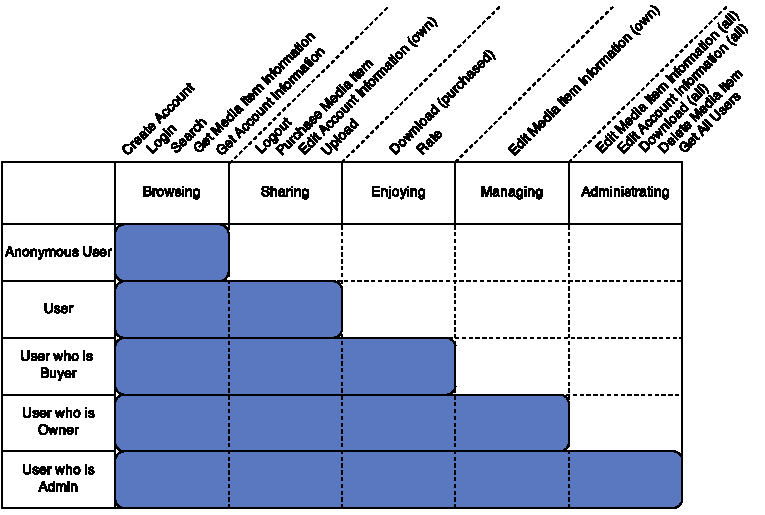
\includegraphics{AccessRightMatrix.pdf}
\caption{Access right matrix for ShareIt}
\label{fig:accessrightmatrix}
\end{figure}

Every call to a service that requires a logged in user therefore validates the user credentials in order to determine whether the user credentials are accepted by \textit{ShareIt} (as discussed in section~\ref{sec:UserCredential}) and if so whether the requesting user has the fitting type of access right. The method responsible for checking the access right takes both the id of the user and the id of media item as parameters. The return type is the enum (read more about enums in section~\ref{sec:enums}) \texttt{AccessRightType} and the method has the following signature:

\begin{lstlisting}
   AccessRightType CheckUserAccess(int userId, int mediaItemId);
\end{lstlisting}


If the user credentials are not accepted an \texttt{InvalidUserException} is thrown, while an \texttt{Unauthorized- UserException} is thrown if no fitting access right exists. 

\end{document}